% Options for packages loaded elsewhere
\PassOptionsToPackage{unicode}{hyperref}
\PassOptionsToPackage{hyphens}{url}
\PassOptionsToPackage{dvipsnames,svgnames,x11names}{xcolor}
%
\documentclass[
  number,
  preprint,
  3p,
  twocolumn]{elsarticle}

\usepackage{amsmath,amssymb}
\usepackage{iftex}
\ifPDFTeX
  \usepackage[T1]{fontenc}
  \usepackage[utf8]{inputenc}
  \usepackage{textcomp} % provide euro and other symbols
\else % if luatex or xetex
  \usepackage{unicode-math}
  \defaultfontfeatures{Scale=MatchLowercase}
  \defaultfontfeatures[\rmfamily]{Ligatures=TeX,Scale=1}
\fi
\usepackage{lmodern}
\ifPDFTeX\else  
    % xetex/luatex font selection
\fi
% Use upquote if available, for straight quotes in verbatim environments
\IfFileExists{upquote.sty}{\usepackage{upquote}}{}
\IfFileExists{microtype.sty}{% use microtype if available
  \usepackage[]{microtype}
  \UseMicrotypeSet[protrusion]{basicmath} % disable protrusion for tt fonts
}{}
\makeatletter
\@ifundefined{KOMAClassName}{% if non-KOMA class
  \IfFileExists{parskip.sty}{%
    \usepackage{parskip}
  }{% else
    \setlength{\parindent}{0pt}
    \setlength{\parskip}{6pt plus 2pt minus 1pt}}
}{% if KOMA class
  \KOMAoptions{parskip=half}}
\makeatother
\usepackage{xcolor}
\setlength{\emergencystretch}{3em} % prevent overfull lines
\setcounter{secnumdepth}{5}
% Make \paragraph and \subparagraph free-standing
\ifx\paragraph\undefined\else
  \let\oldparagraph\paragraph
  \renewcommand{\paragraph}[1]{\oldparagraph{#1}\mbox{}}
\fi
\ifx\subparagraph\undefined\else
  \let\oldsubparagraph\subparagraph
  \renewcommand{\subparagraph}[1]{\oldsubparagraph{#1}\mbox{}}
\fi

\usepackage{color}
\usepackage{fancyvrb}
\newcommand{\VerbBar}{|}
\newcommand{\VERB}{\Verb[commandchars=\\\{\}]}
\DefineVerbatimEnvironment{Highlighting}{Verbatim}{commandchars=\\\{\}}
% Add ',fontsize=\small' for more characters per line
\usepackage{framed}
\definecolor{shadecolor}{RGB}{241,243,245}
\newenvironment{Shaded}{\begin{snugshade}}{\end{snugshade}}
\newcommand{\AlertTok}[1]{\textcolor[rgb]{0.68,0.00,0.00}{#1}}
\newcommand{\AnnotationTok}[1]{\textcolor[rgb]{0.37,0.37,0.37}{#1}}
\newcommand{\AttributeTok}[1]{\textcolor[rgb]{0.40,0.45,0.13}{#1}}
\newcommand{\BaseNTok}[1]{\textcolor[rgb]{0.68,0.00,0.00}{#1}}
\newcommand{\BuiltInTok}[1]{\textcolor[rgb]{0.00,0.23,0.31}{#1}}
\newcommand{\CharTok}[1]{\textcolor[rgb]{0.13,0.47,0.30}{#1}}
\newcommand{\CommentTok}[1]{\textcolor[rgb]{0.37,0.37,0.37}{#1}}
\newcommand{\CommentVarTok}[1]{\textcolor[rgb]{0.37,0.37,0.37}{\textit{#1}}}
\newcommand{\ConstantTok}[1]{\textcolor[rgb]{0.56,0.35,0.01}{#1}}
\newcommand{\ControlFlowTok}[1]{\textcolor[rgb]{0.00,0.23,0.31}{#1}}
\newcommand{\DataTypeTok}[1]{\textcolor[rgb]{0.68,0.00,0.00}{#1}}
\newcommand{\DecValTok}[1]{\textcolor[rgb]{0.68,0.00,0.00}{#1}}
\newcommand{\DocumentationTok}[1]{\textcolor[rgb]{0.37,0.37,0.37}{\textit{#1}}}
\newcommand{\ErrorTok}[1]{\textcolor[rgb]{0.68,0.00,0.00}{#1}}
\newcommand{\ExtensionTok}[1]{\textcolor[rgb]{0.00,0.23,0.31}{#1}}
\newcommand{\FloatTok}[1]{\textcolor[rgb]{0.68,0.00,0.00}{#1}}
\newcommand{\FunctionTok}[1]{\textcolor[rgb]{0.28,0.35,0.67}{#1}}
\newcommand{\ImportTok}[1]{\textcolor[rgb]{0.00,0.46,0.62}{#1}}
\newcommand{\InformationTok}[1]{\textcolor[rgb]{0.37,0.37,0.37}{#1}}
\newcommand{\KeywordTok}[1]{\textcolor[rgb]{0.00,0.23,0.31}{#1}}
\newcommand{\NormalTok}[1]{\textcolor[rgb]{0.00,0.23,0.31}{#1}}
\newcommand{\OperatorTok}[1]{\textcolor[rgb]{0.37,0.37,0.37}{#1}}
\newcommand{\OtherTok}[1]{\textcolor[rgb]{0.00,0.23,0.31}{#1}}
\newcommand{\PreprocessorTok}[1]{\textcolor[rgb]{0.68,0.00,0.00}{#1}}
\newcommand{\RegionMarkerTok}[1]{\textcolor[rgb]{0.00,0.23,0.31}{#1}}
\newcommand{\SpecialCharTok}[1]{\textcolor[rgb]{0.37,0.37,0.37}{#1}}
\newcommand{\SpecialStringTok}[1]{\textcolor[rgb]{0.13,0.47,0.30}{#1}}
\newcommand{\StringTok}[1]{\textcolor[rgb]{0.13,0.47,0.30}{#1}}
\newcommand{\VariableTok}[1]{\textcolor[rgb]{0.07,0.07,0.07}{#1}}
\newcommand{\VerbatimStringTok}[1]{\textcolor[rgb]{0.13,0.47,0.30}{#1}}
\newcommand{\WarningTok}[1]{\textcolor[rgb]{0.37,0.37,0.37}{\textit{#1}}}

\providecommand{\tightlist}{%
  \setlength{\itemsep}{0pt}\setlength{\parskip}{0pt}}\usepackage{longtable,booktabs,array}
\usepackage{calc} % for calculating minipage widths
% Correct order of tables after \paragraph or \subparagraph
\usepackage{etoolbox}
\makeatletter
\patchcmd\longtable{\par}{\if@noskipsec\mbox{}\fi\par}{}{}
\makeatother
% Allow footnotes in longtable head/foot
\IfFileExists{footnotehyper.sty}{\usepackage{footnotehyper}}{\usepackage{footnote}}
\makesavenoteenv{longtable}
\usepackage{graphicx}
\makeatletter
\def\maxwidth{\ifdim\Gin@nat@width>\linewidth\linewidth\else\Gin@nat@width\fi}
\def\maxheight{\ifdim\Gin@nat@height>\textheight\textheight\else\Gin@nat@height\fi}
\makeatother
% Scale images if necessary, so that they will not overflow the page
% margins by default, and it is still possible to overwrite the defaults
% using explicit options in \includegraphics[width, height, ...]{}
\setkeys{Gin}{width=\maxwidth,height=\maxheight,keepaspectratio}
% Set default figure placement to htbp
\makeatletter
\def\fps@figure{htbp}
\makeatother

\makeatletter
\@ifpackageloaded{caption}{}{\usepackage{caption}}
\AtBeginDocument{%
\ifdefined\contentsname
  \renewcommand*\contentsname{Table of contents}
\else
  \newcommand\contentsname{Table of contents}
\fi
\ifdefined\listfigurename
  \renewcommand*\listfigurename{List of Figures}
\else
  \newcommand\listfigurename{List of Figures}
\fi
\ifdefined\listtablename
  \renewcommand*\listtablename{List of Tables}
\else
  \newcommand\listtablename{List of Tables}
\fi
\ifdefined\figurename
  \renewcommand*\figurename{Figure}
\else
  \newcommand\figurename{Figure}
\fi
\ifdefined\tablename
  \renewcommand*\tablename{Table}
\else
  \newcommand\tablename{Table}
\fi
}
\@ifpackageloaded{float}{}{\usepackage{float}}
\floatstyle{ruled}
\@ifundefined{c@chapter}{\newfloat{codelisting}{h}{lop}}{\newfloat{codelisting}{h}{lop}[chapter]}
\floatname{codelisting}{Listing}
\newcommand*\listoflistings{\listof{codelisting}{List of Listings}}
\makeatother
\makeatletter
\makeatother
\makeatletter
\@ifpackageloaded{caption}{}{\usepackage{caption}}
\@ifpackageloaded{subcaption}{}{\usepackage{subcaption}}
\makeatother
\usepackage{float}
\makeatletter
\let\oldlt\longtable
\let\endoldlt\endlongtable
\def\longtable{\@ifnextchar[\longtable@i \longtable@ii}
\def\longtable@i[#1]{\begin{figure}[H]
\onecolumn
\begin{minipage}{0.5\textwidth}
\oldlt[#1]
}
\def\longtable@ii{\begin{figure}[H]
\onecolumn
\begin{minipage}{0.5\textwidth}
\oldlt
}
\def\endlongtable{\endoldlt
\end{minipage}
\twocolumn
\end{figure}}
\makeatother
\ifLuaTeX
  \usepackage{selnolig}  % disable illegal ligatures
\fi
\usepackage[]{natbib}
\bibliographystyle{elsarticle-num}
\usepackage{bookmark}

\IfFileExists{xurl.sty}{\usepackage{xurl}}{} % add URL line breaks if available
\urlstyle{same} % disable monospaced font for URLs
\hypersetup{
  pdftitle={Predecir la popularidad de noticias en línea utilizando modelos de clasificación y/o regresión},
  pdfauthor={Calderon, S., Arenas, K., Torres, J.},
  colorlinks=true,
  linkcolor={blue},
  filecolor={Maroon},
  citecolor={Blue},
  urlcolor={Blue},
  pdfcreator={LaTeX via pandoc}}

\setlength{\parindent}{6pt}
\begin{document}

\begin{frontmatter}
\title{Predecir la popularidad de noticias en línea utilizando modelos
de clasificación y/o regresión}
\author[]{Calderon, S., Arenas, K., Torres, J.%
%
}



\cortext[cor1]{Corresponding author}

        





\end{frontmatter}
    
\section{Resumen}\label{resumen}

\section{Introducción}\label{introducciuxf3n}

El estudio de la popularidad de las noticias en línea ha cobrado gran
relevancia en la última década, ya que los medios compiten por la
atención en un entorno digital saturado. La capacidad de predecir qué
noticias serán populares es esencial para optimizar estrategias de
contenido y aumentar la participación de la audiencia. Para abordar este
desafío, se han desarrollado modelos basados en datos históricos y
aprendizaje automático que consideran una variedad de características,
como el contenido de la noticia, el comportamiento del usuario y las
dinámicas de las plataformas de distribución. Los usuarios, quienes son
los consumidores de estos medios usualmente comparten, se suscriben e
interactúan con la información. La noción de popularidad suele
expresarse investigando el número de interacciones en la web y las redes
sociales, por ejemplo, la tasa de clics, el número de compartidos, me
gusta y retweets \citep{Uddin2016}. El número de veces que se comparte
una noticia es un buen indicador de su popularidad potencial. La
predicción de la popularidad de un artículo tiene múltiples aplicaciones
en el mundo real, desde el punto de vista de \citep{Tarar2014a}, hay dos
caminos de predicción más conocidas: el primero relacionado con las
características que se conocen luego de la publicación y los que no
utilizan dichas características. El primero es el más conocido y más
común
\citep{Kaltenbrunner2007, Szabo2010, Lee2012, Ahmed2013, Tatar2014b}. De
acuerdo a \citep{Fernandes2015}, la popularidad de un artículo candidato
puede ser estimado utilizando un módulo de predicción y luego un módulo
de optimización, según el autor sugiere cambios en el contenido y la
estructura del artículo, con el fin de maximizar su popularidad
esperada. Existen varios estudios que sugieren, la predicción puede ser
alta utilizando los metadatos posteriores a la publicación, dándonos
ventaja en la atención recibidas de la información luego de ser recibida
\citep{Lee2012, Ahmed2013}. Por el contrario \citep{Fernandes2015},
menciona que al utilizar las características de metadatos antes de la
publicación de los contenidos resulta ser difícil, aunque la precisión
de la predicción esperada es comparativamente baja en el método de antes
de la publicación, ya que estamos utilizando sólo características de
metadatos en lugar del contenido original de la noticia.

El objetivo de este artículo es desarrollar un modelo de aprendizaje
automático que logre predecir la popularidad de los artículos de
noticias en línea antes de su publicación. La sección de estado del arte
presenta trabajos previos en la materia, incluyendo la metodología y
resultados. La sección Diseño del experimento se centra en explicar la
metodología de este artículo, incluyendo la descripción del conjunto de
datos y los modelos a ser entrenados.

\section{Estado del arte}\label{estado-del-arte}

Esta sección proporciona un resumen cohesivo de estudios de
investigación enfocados en medir y predecir la popularidad de los
artículos de noticias en línea. Los dos primeros estudios abordan los
desafíos de predecir la popularidad de las noticias en el momento de su
publicación, mientras que los últimos tres profundizan en la aplicación
de técnicas de aprendizaje automático en un único conjunto de datos para
mejorar las capacidades predictivas de la popularidad de los artículos
de noticias.

\citep{arapakis2014} investiga las dificultades asociadas con predecir
la popularidad de los artículos de noticias inmediatamente después de su
publicación. Utilizando un conjunto de datos de 13,319 artículos de
Yahoo News, los autores critican investigaciones previas, que afirmaban
una alta precisión en la predicción de la popularidad de las noticias
utilizando características basadas en el contenido. Se argumenta que la
tarea es más compleja de lo que se pensaba, principalmente debido a la
alta asimetría en la distribución de popularidad. Sus experimentos
revelan que los métodos de clasificación y regresión existentes están
sesgados hacia la predicción de artículos impopulares, fallando en
identificar con precisión los populares, que son cruciales para la
identificación temprana. El estudio concluye que los métodos actuales
son inadecuados para predecir la popularidad de las noticias desde el
inicio utilizando solo características basadas en el contenido,
destacando la necesidad de enfoques más robustos.

En \citep{hensinger2012}, los autores abordan el desafío de predecir qué
artículos de noticias aparecerán en una lista de ``más leídos''.
Proponen que la popularidad es un concepto relativo influenciado por el
atractivo de los artículos publicados simultáneamente. Empleando una
función lineal en una representación de bolsa de palabras, utilizan
Máquinas de Soporte Vectorial de Ranking (Ranking SVMs) entrenadas en
pares de artículos de la misma fecha y medio. El modelo, que utiliza
información mínima como contenido textual, fechas de publicación y
estado de popularidad, predice con éxito los artículos populares e
identifica palabras clave influyentes. Utilizando un conjunto de datos
de diez medios importantes en inglés durante un año, el estudio logra
precisiones que a menudo superan el 60\%, superando los métodos de
clasificación binaria. Esta investigación destaca la naturaleza dinámica
del atractivo de las noticias y proporciona un marco robusto para
predecir la popularidad de las noticias.

En \citep{fernandes2015}, se introduce un Sistema Proactivo de Soporte
de Decisiones Inteligente (IDSS) está diseñado para predecir la
popularidad de los artículos de noticias en línea antes de su
publicación. Utilizando un conjunto de datos de 39,000 artículos del
sitio web Mashable, el IDSS aprovecha diversas características,
incluyendo contenido digital, popularidad de noticias referenciadas,
participación de palabras clave y análisis de sentimientos. El sistema
emplea modelos de aprendizaje automático como Bosques Aleatorios (Random
Forest), Adaptive Boosting y Máquinas de Soporte Vectorial (SVM) para
una tarea de clasificación binaria. El modelo Random Forest alcanza un
poder de discriminación del 73\%, mientras que un módulo de optimización
que utiliza búsqueda local por escalada estocástica mejora la
probabilidad de popularidad estimada en 15 puntos porcentuales. El IDSS
no solo predice, sino que también sugiere modificaciones en el contenido
y la estructura del artículo para mejorar la popularidad esperada,
demostrando ser una herramienta valiosa para los autores de noticias en
línea.

Usando el mismo conjunto de datos, \citep{Ren2015PredictingAE} evalúa
diversas técnicas de aprendizaje automático para predecir la popularidad
de los artículos de noticias en línea. Se obtuvieron conocimientos
iniciales utilizando regresión lineal y logística, logrando la regresión
logística una precisión del 66\% al categorizar la variable objetivo en
categorías binarias. Usando SVM, los autores enfrentaron inicialmente
problemas de alto sesgo, pero mostraron mejoras marginales con núcleos
más complejos, alcanzando una precisión del 55\%. Sin embargo, el modelo
de Random Forest emergió como el más efectivo, logrando una precisión
del 70\% con parámetros óptimos. Al aprovechar múltiples árboles de
decisión y subconjuntos de características, Random Forest mitigó
eficazmente la varianza, proporcionando las predicciones más precisas.

Finalmente, \citep{khan2018} explora la predicción de la popularidad de
artículos de noticias utilizando el conjunto de datos de Mashable
mediante diversas técnicas de aprendizaje automático. Se aplicaron
métodos de selección de características como la selección univariada, la
eliminación recursiva de características y el análisis de componentes
principales para identificar las características más relevantes que
influyen en la popularidad de los artículos. Evaluaron once modelos de
clasificación, incluidos Naïve Bayes, regresión logística, árboles de
decisión, redes neuronales, bosques aleatorios y máquinas de vectores de
soporte. Entre estos, el método de potenciación del gradiente (gradient
boosting) surgió como el modelo más eficaz, logrando una precisión del
79.7\%. El estudio concluyó que los métodos en ensamble, en particular
gradient boosting, son los que mejor funcionan para predecir la
popularidad de los artículos de noticias.

Esta colección de investigaciones destaca las complejidades y avances en
la predicción de la popularidad de las noticias en línea. La predicción
temprana desde el inicio sigue siendo un desafío debido a las
distribuciones de popularidad sesgadas y los sesgos de los modelos. Sin
embargo, las técnicas sofisticadas de aprendizaje automático y las
estrategias exhaustivas de preprocesamiento muestran promesas para
mejorar la precisión de la predicción. La investigación y desarrollo
continuos de metodologías robustas son cruciales para futuros avances en
este dominio.

\section{Diseño del experimento}\label{diseuxf1o-del-experimento}

Para este estudio, se utilizará el conjunto de datos elaborado en
\citep{fernandes2015}. Cuenta con 59 características y una columna
target. esta última contiene información de las veces que el artículo
fue compartido (numérica), siendo esta la medición de popularidad. En
general, el conjunto de datos permite un análisis exhaustivo de las
características del contenido, la participación del usuario y la
efectividad de varios tipos de contenido a lo largo de diferentes
canales y en el tiempo. A continuación, se presenta una descripción más
detallada.

\subsection{Descripción del conjunto de datos (falta
completar)}\label{descripciuxf3n-del-conjunto-de-datos-falta-completar}

El conjunto de datos proporciona una visión general exhaustiva del
contenido en línea, incorporando varias métricas y características
relacionadas con atributos textuales, elementos multimedia e indicadores
de participación. Captura atributos textuales clave, como el número de
tokens en los títulos y el contenido, la proporción de tokens únicos y
la longitud promedio de los tokens, ofreciendo información sobre la
complejidad y estructura del contenido. El conjunto de datos también
incluye métricas de palabras clave, que destacan la relevancia e
importancia de las palabras clave en el contenido. Además, registra el
número de hipervínculos y elementos multimedia como imágenes y videos,
reflejando la riqueza y los aspectos multimedia de los artículos o
publicaciones.

Además, el conjunto de datos clasifica el contenido en diferentes
canales, como estilo de vida, entretenimiento, negocios, redes sociales,
tecnología y noticias mundiales, proporcionando una clara clasificación
de los tipos de contenido. Se incluye información temporal a través de
variables que indican el día de la semana en que se publicó el contenido
y si se publicó en un fin de semana. En estos casos, las variables han
sido incluidas como binarias.

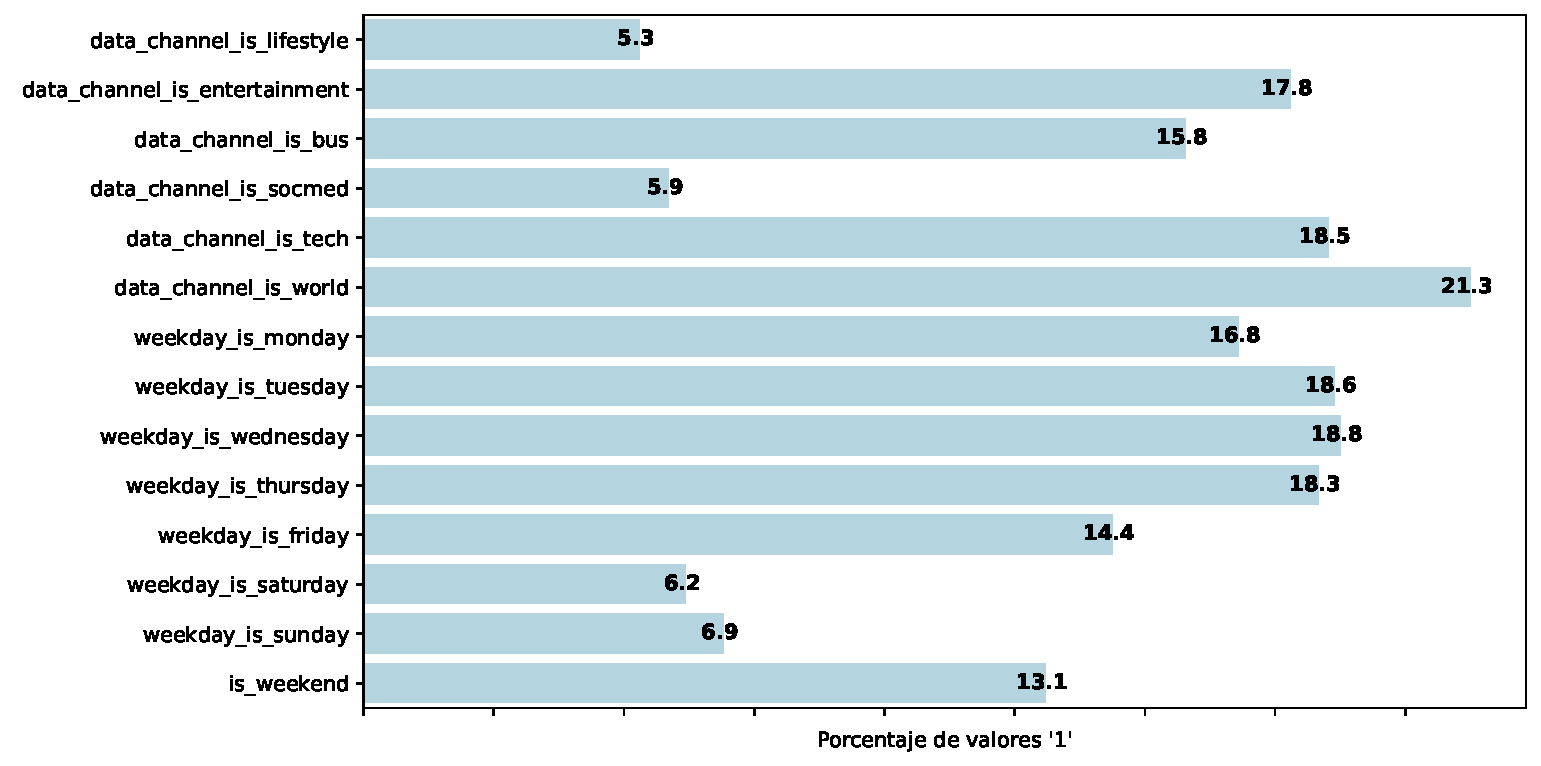
\includegraphics{Articulo_v2_files/figure-pdf/cell-4-output-1.pdf}

El conjunto de datos también presenta componentes de análisis semántico
latente y puntuaciones de sentimiento, capturando el tono emocional y la
objetividad del contenido. Las métricas de participación, como el número
de veces que se comparte y las referencias a sí mismo, son cruciales
para comprender el alcance e impacto del contenido. Todas estas son
variables continuas.

\subsection{Metodología}\label{metodologuxeda}

El presente trabajo se prioriza en el procesamiento de los datos y
esencialmente antes del entrenamiento de los datos. Por tanto, se
seguirá los siguientes pasos:

\#1) Preparación de datos, este punto realizaremos la limpieza de datos,
el manejo de valores faltantes, nulos y detección de los outlier.

\begin{enumerate}
\def\labelenumi{\arabic{enumi})}
\setcounter{enumi}{1}
\tightlist
\item
  Exploración y análisis de datos: en este paso realizaremos la
  reducción de la dimensionalidad utilizando la herramienta de análisis
  de principales componentes (PCA) y análisis de correlación de datos,
  ambos métodos nos ayudaran a visualizar y entender las relaciones y
  patrones de las variables.
\end{enumerate}

PCA, toma encuenta la varianza ya incluye el analis de correlacion

\begin{enumerate}
\def\labelenumi{\arabic{enumi})}
\setcounter{enumi}{2}
\tightlist
\item
  Selección y entrenamiento del modelo; los datos clasificacion:
  `RandomForest': RandomForestClassifier(), `AdaBoost':
  AdaBoostClassifier(), `LogisticRegression': LogisticRegression()
  GridSearchCV gradienBoots Redes neuronales (opcional)
\end{enumerate}

considerando que los datos se acomodan para aplicar modelos de
regresión, priorizaremos la metodología de , el cual es una técnica que
se utiliza la mejor combinación de hiperparámetros. En este punto,
además, optimizaremos los parámetros del modelo para mejorar su
rendimiento.

\begin{enumerate}
\def\labelenumi{\arabic{enumi})}
\setcounter{enumi}{3}
\item
  En seguida realizaremos la validación y evaluación del modelo: en
  otras palabras, medir el rendimiento del modelo utilizando datos de
  prueba y métricas de evaluación. Aquiursasi y el area bajo la curva
\item
  Finalmente se describirá los resultados, interpretación y discusiones:
  en esta parte nos apoyaremos mediante figuras y gráficos estadísticos
  y correlacionaremos con anteriores resultados.
\end{enumerate}

\section{Experimentación y
resultados}\label{experimentaciuxf3n-y-resultados}

\section{Referencias}\label{referencias}

\section{Quarto}\label{quarto}

Quarto enables you to weave together content and executable code into a
finished document. To learn more about Quarto see
\url{https://quarto.org}.

\section{Running Code}\label{running-code}

When you click the \textbf{Render} button a document will be generated
that includes both content and the output of embedded code. You can
embed code like this:

\begin{verbatim}
2
\end{verbatim}

You can add options to executable code like this

\begin{verbatim}
4
\end{verbatim}

The \texttt{echo:\ false} option disables the printing of code (only
output is displayed). This is the default behavior.

When you use \texttt{echo:\ true} you will show both the code and the
output.

\begin{Shaded}
\begin{Highlighting}[]
\BuiltInTok{print}\NormalTok{(}\StringTok{"Hello"}\NormalTok{)}
\end{Highlighting}
\end{Shaded}

\begin{verbatim}
Hello
\end{verbatim}

\section{Using figures and equations}\label{using-figures-and-equations}

Using \texttt{fig-cap} allows you to specifiy a caption for a figure.
Use it in code blocks where the last line prints a plot.

\begin{figure}

\centering{

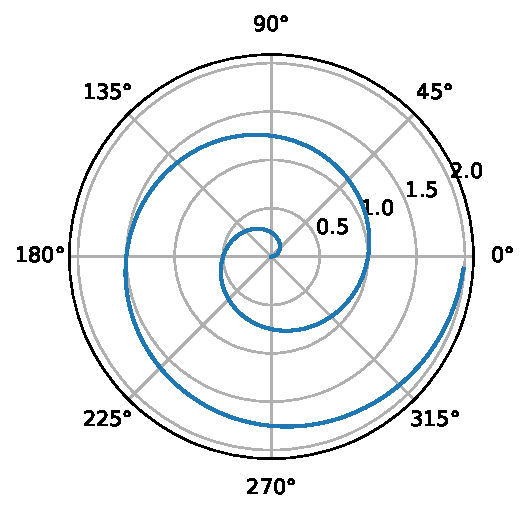
\includegraphics{Articulo_v2_files/figure-pdf/fig-radial-output-1.pdf}

}

\caption{\label{fig-radial}Radial plot}

\end{figure}%

You can write Latex equiations:

\[
E=mc^2
\]

If the label attribute of a code chunk starts with \texttt{fig-} when it
renders a plot, you can reference it. For example, here we reference
Figure~\ref{fig-radial}.

Be attentive as some things might need manual tweaking.

\section{Using other formating}\label{using-other-formating}

Multiple formatting options

\begin{enumerate}
\def\labelenumi{\arabic{enumi}.}
\tightlist
\item
  You can use lists
\item
  They will numerate by themselves
\item
  No need to worry about counting
\end{enumerate}

You are not restricted to numbered lists.

\begin{itemize}
\tightlist
\item
  first
\item
  second
\item
  third
\end{itemize}

\subsection{Use of sub headers}\label{use-of-sub-headers}

Organize your document as you please. How much organization do you
really need?

\subsection{Another subheader}\label{another-subheader}

Does this looks nice to you? This document follows Markdown conventions.

\subsubsection{A deeper level}\label{a-deeper-level}

However, is best that you don't go too deep because lower levels might
not be fully supported in this template.

\section{Citations}\label{citations}

You can add citationsfor something some said at some point. Your
references should be inside the \texttt{references.bib} file. Some
people might have already researched this field
\citep[see][pp.~1-2]{misc_online_news_popularity_332}.


\renewcommand\refname{References}
  \bibliography{references.bib}


\end{document}
